\documentclass{standalone}

\usepackage{tikz}
\usepackage{tikz-3dplot}

\begin{document}

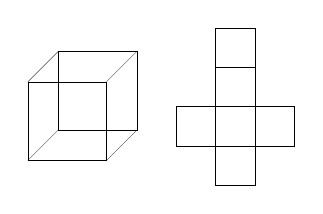
\begin{tikzpicture}

    % 绘制三维正方体
    \tdplotsetmaincoords{30}{30} % 设置视角
    % 画正方体的边,使用 ultra thin
    \draw[ultra thin] (0,0,0) -- (1,0,0) -- (1,1,0) -- (0,1,0) -- cycle; % 底面
    \draw[ultra thin] (0,0,1) -- (1,0,1) -- (1,1,1) -- (0,1,1) -- cycle; % 顶面
    \draw[ultra thin] (0,0,0) -- (0,0,1); % 前左边
    \draw[ultra thin] (1,0,0) -- (1,0,1); % 前右边
    \draw[ultra thin] (1,1,0) -- (1,1,1); % 后右边
    \draw[ultra thin] (0,1,0) -- (0,1,1); % 后左边

    % 移动到右侧绘制展开图
    \begin{scope}[xshift=2cm,yshift=-0.7cm,scale=.5]
        % 绘制正方体的展开图(十字架样式)
        \draw[ultra thin] (0,0) rectangle (1,4);   % 中间面
        \draw[ultra thin] (-1,1) rectangle (2,2);   % 上面
        \draw[ultra thin] (0,3) -- (1,3);
    \end{scope}

\end{tikzpicture}

\end{document}
